% Nome do capítulo
\chapter{Trabalhos Relacionados}
\label{cap:3}
\vspace{-1.9cm}

\section{\textit{\ac{DenseNet}}}

Como mencionado anteriormente, desde 2012 as tarefas de classificação de imagens são resolvidas majoritariamente por arquiteturas de \textit{Deep Learning}. \citeonline{he-2016} propôs uma nova arquitetura que utilizava o conceito de \textit{skip connection}, que, como explicado anteriormente, consiste em utilizar a saída de uma camada em camadas posteriores além da próxima. O conceito de \textit{skip connection} fez tanto sucesso que tornou a ser utilizado em um modelo mais recente. \cite{liu-2017} propuseram um modelo de \ac{CNN} que utiliza esse mesmo conceito, porém de uma forma um pouco diferente. 

Nas \ac{ResNet}s, existem os blocos residuais, conforme a figura \ref{fig:blocoresidual}. No bloco residual temos duas camadas $c_1$ e $c_2$ onde $c_1$ é a entrada de $c_2$. Na saída deste bloco residual será feita uma soma de matrizes entre as saídas de $c_1$ e $c_2$ e essa soma será usada na entrada das camadas posteriores. 

Nas \ac{DenseNet}s, o conceito de skip connection é utilizado conforme a figura \ref{fig:blocodenso}. Um bloco denso $B$ composto por um conjunto de camadas $C = \{c_1, c_2, ..., c_n\}$ onde $c_1$ é a entrada de $c_2$. A primeira diferença é que para as camadas sucessoras, todas as camadas anteriores estarão na entrada, isso é, a entrada de $c_3$ será $\{c_1, c_2\}$, a entrada de $c_4$ será $\{c_1, c_2,c_3\}$ e assim sucessivamente. A segunda diferença é que nos blocos densos as saídas das camadas são unidas por uma concatenação de matrizes, não por soma. Sendo assim, se cada camada do bloco possui uma saída de $x$ matrizes, o bloco possui $n$ camadas e a entrada do bloco possui tamanho $a$, a saída possuirá o tamanho representado pela equação \ref{eq:eq8}:

\begin{equation}
	\label{eq:eq8}	y = n x + a
\end{equation}

Vale mencionar que o valor de $x$ se conserva para toda a rede. Uma vantagem de usar blocos densos é a possibilidade de propagar informações com diversos níveis de abstração ao longo de toda a rede.

As \ac{DenseNet}s seguem um padrão arquitetural muito similar ao das \ac{ResNet}s começando a rede com uma camada de convolução $7\times7$ com \textit{strides} de $2\times2$ que é sucedida por uma camada de \textit{batch normalization} e outra de \ac{ReLU}. Depois disso, têm uma camada de \textit{pooling} máximo e após essa camada, tem quatro blocos densos intercalados por blocos intermediários. Os blocos de convolução dentro dos blocos densos são compostos por uma camada de convolução $1\times1$ (que \citeauthor{liu-2017} definem como camada de ``gargalo'') e uma camada de convolução $3\times3$. Vale mencionar que todas as camadas de convolução nos blocos densos são precedidas por uma camada de \textit{batch normalization} e \ac{ReLU}. Os blocos intermediários são compostos por uma camada de convolução $1\times1$ seguida de uma camada de \textit{pooling} médio (que também é precedida por \textit{batch normalization} e \ac{ReLU}). No final dos 4 blocos densos, a rede possui mais uma camada de \textit{batch normalization} e \ac{ReLU} seguida por um \textit{pooling} médio global e uma camada completamente conectada que faz a classificação. A figura \ref{fig:archdensenet} mostra como é a arquitetura da rede.

\begin{figure}[H]
	% Alterar espaçamentos antes e depois do caption
	\setlength{\abovecaptionskip}{0pt}
	\setlength{\belowcaptionskip}{0pt}
	% Caption
	\caption[Exemplo de bloco denso]{Exemplo de bloco denso}
	\centering
	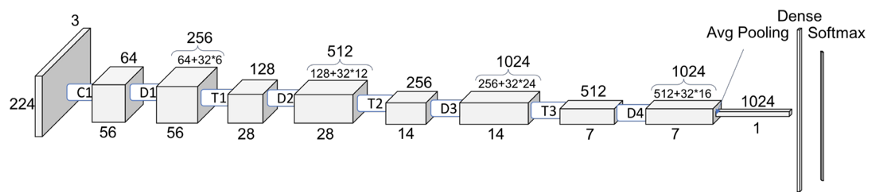
\includegraphics[width=.7\textwidth]{imagem/0x_densenet_arch.png}
	% Caption centralizada
	\captionsetup{justification=centering}
	\captionfont{\small{\textbf{\\Fonte: \citeonline{liu-2017}.}}}	
	\label{fig:archdensenet}
\end{figure}

O modelo proposto obteve resultados competitivos com os da literatura, ficando em segundo lugar no \ac{ILSVRC} de 2017 e apresentando resultados competitivos com os da literatura na época. O artigo também foi premiado como a melhor publicação da \ac{CVPR} do ano de 2017. O modelo obteve uma acurácia de 96\% na cifar-10 e 82\% na cifar-100.

\section{SSD: \textit{Single-Shot Multibox Detector}}

\citeonline{wei-2015} propuseram um método a base de redes neurais convolucionais para fazer a localização e detecção de objetos. A proposta deles melhorou significativamente os resultados apresentados no estado da arte. Isso se deve ao fato de que eles não só conseguiram propor um modelo que faz a localização e classificação de forma eficiente (chegando a 74,3\% de acurácia), como conseguiram obter esse resultado fazendo classificação e localização em tempo real, com uma velocidade de 59 \ac{FPS}. Uma outra vantagem obtida por esse método é que ele consegue fazer a localização e classificação em imagens significativamente menores, uma vez que os quadros processados pelo \ac{YOLO} têm dimensões $448 \times 448$ e os processados pelo \ac{R-CNN} têm $1000\times 600$, o \ac{SSD} processa quadros de dimensões $300 \times 300$. Isso é uma vantagem, pois mesmo o algoritmo trabalhando com imagens menores, o resultado consegue competir com os outros métodos.

A abordagem consiste em utilizar a rede VGG16 \cite{simonyan-2014} como arquitetura base, substituir as camadas completamente conectadas fc6 e fc7 por camadas convolucionais, alterar o filtro pool5 de $2 \times 2 - s2$ para $3 \times 3 - s1$, e usaram o algoritmo \textit{à trous}\cite{holschneider-1990} para preencher os espaços vazios. Além disso, eles removeram todas as camadas de \textit{dropout} e a última camada completamente conectada. Por fim, as camadas de convolução geram os resultados de mais de 8000 localizações e classificações, as quais são filtradas em um passo final de supressão de não-máximos, que elimina todos os resultados com confiança abaixo de $0,5$.

  \begin{figure}[H]
	% Alterar espaçamentos antes e depois do caption
	\setlength{\abovecaptionskip}{0pt}
	\setlength{\belowcaptionskip}{0pt}
	% Caption
	\caption[YOLO e SSD]{Comparação entre \ac{YOLO} e \ac{SSD}}
	\centering
	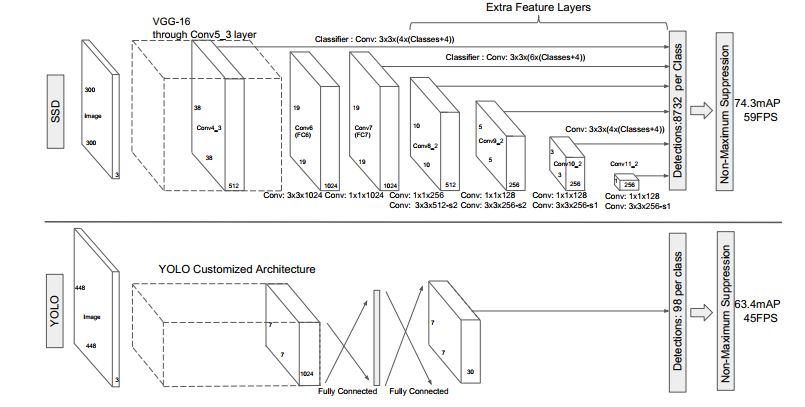
\includegraphics[width=.6\textwidth]{imagem/0x_yoloxssd.JPG}
	% Caption centralizada
	\captionsetup{justification=centering}
	\captionfont{\small{\textbf{\\Fonte: \citeonline{wei-2015}.}}}	
	\label{fig:yoloxssd}
\end{figure}

A Figura \ref{fig:yoloxssd} mostra as diferenças entre as arquiteturas \ac{YOLO} e \ac{SSD}. Enquanto \citeonline{redmon-2015} usaram uma camada completamente conectada intermediária para fazer a localização dos objetos, \citeonline{wei-2015} usaram camadas de convolução sobre mapas de múltiplos tamanhos. Além disso, o \ac{SSD} trabalha com \textit{bounding-boxes} de tamanhos padrões $\{1, 2, 3, \frac{1}{2}, \frac{1}{3}\}$. Os filtros de convolução adicionais, os tamanhos padrões de \textit{bounding-boxes} e o uso de \textit{data-augmentation} foram cruciais na obtenção dos bons resultados.

\section{DSSD: \textit{Deconvolution Single-Shot Detector}}

\citeonline{cheng-2017} propuseram uma extensão do \ac{SSD}. Depois dos resultados obtidos pelo \ac{SSD} ao fazer localizção e classificação de objetos com uma acurácia de $79,5\%$, eles propuseram uma abordagem alternativa, usando camadas de deconvolução ao final da rede. As camadas de deconvolução tem entre seus resultados o aumento de resolução do mapa de entrada. A abordagem visou explorar esse efeito com o intuito de aumentar a acurácia da classificação e localização de objetos, e, com isso, atingir uma acurácia de $81,5\%$. Embora essa abordagem tenha uma acurácia maior do que a obtida por \citeonline{wei-2015}, ela não é rápida o bastante pra fazer localização e classificação em tempo real.


\begin{figure}[H]
	% Alterar espaçamentos antes e depois do caption
	\setlength{\abovecaptionskip}{0pt}
	\setlength{\belowcaptionskip}{0pt}
	% Caption
	\caption[SSD e DSSD]{Comparação entre \ac{SSD} e \ac{DSSD}}
	\centering
	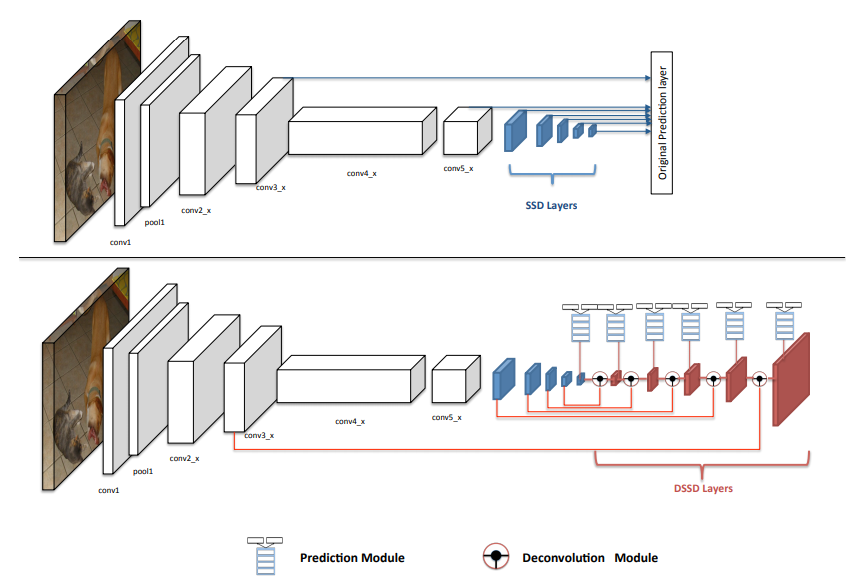
\includegraphics[width=.8\textwidth]{imagem/0x_comparacao_ssd_dssd.png}
	% Caption centralizada
	\captionsetup{justification=centering}
	\captionfont{\small{\textbf{\\Fonte: \citeonline{cheng-2017}.}}}	
	\label{fig:ssdxdssd}
\end{figure}

%Rever essa parte
Nesse trabalho, foram propostas duas alterações principais no modelo \ac{SSD}. A primeira delas foi a utilização da rede neural ResNet-101 \citeonline{he-2016} e a segunda foi a utilização das camadas adicionais de deconvolução. Como mostra a Figura \ref{fig:ssdxdssd}, a arquitetura agora também utiliza de módulos de predição individuais, onde a saída da última camada de convolução e a saída de cada camada de deconvolução gera seus próprios resultados para a classificação e localização. A Figura \ref{fig:dssdpred} mostra as variações dos módulos de predição da \ac{DSSD}.

\begin{figure}[H]
	% Alterar espaçamentos antes e depois do caption
	\setlength{\abovecaptionskip}{0pt}
	\setlength{\belowcaptionskip}{0pt}
	% Caption
	\caption[Módulos de predição DSSD]{Módulos de predição \ac{DSSD}}
	\centering
	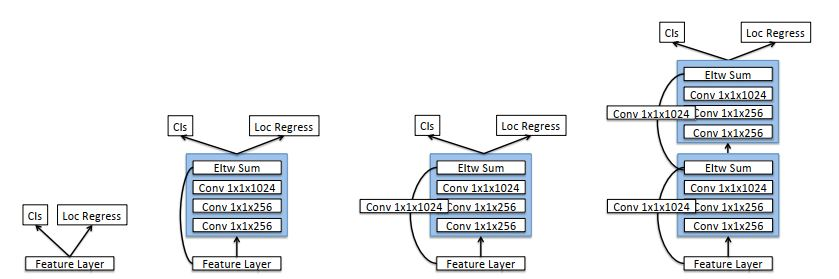
\includegraphics[width=.8\textwidth]{imagem/0x_dssdpredmod.jpg}
	% Caption centralizada
	\captionsetup{justification=centering}
	\captionfont{\small{\textbf{\\Fonte: \citeonline{cheng-2017}.}}}	
	\label{fig:dssdpred}
\end{figure}

Como mencionado anteriormente, embora o \ac{DSSD} tenha melhorado a acurácia do \ac{SSD}, ele não é aplicável para fazer a localização e classificação em tempo real. Com uma acurácia de $81,5\%$ ele consegue processar apenas $6,6$ \ac{FPS}. Isso se deve ao uso das deconvoluções, da ResNet 101 - que possui mais camadas, e, portanto toma mais tempo de processamento - e também ao aumento no número de \textit{bounding boxes} geradas($43688$ vs. $17080$), fazendo assim com que a supressão de não-máximos leve mais tempo.